%SOP Template 
% Version 02 Added revision date
% Version 03 Fixed file/name spelling errors

\documentclass[12pt]{../SOP4_alpha}\usepackage[]{graphicx}\usepackage[]{xcolor}
% maxwidth is the original width if it is less than linewidth
% otherwise use linewidth (to make sure the graphics do not exceed the margin)
\makeatletter
\def\maxwidth{ %
  \ifdim\Gin@nat@width>\linewidth
    \linewidth
  \else
    \Gin@nat@width
  \fi
}
\makeatother

\definecolor{fgcolor}{rgb}{0.345, 0.345, 0.345}
\newcommand{\hlnum}[1]{\textcolor[rgb]{0.686,0.059,0.569}{#1}}%
\newcommand{\hlstr}[1]{\textcolor[rgb]{0.192,0.494,0.8}{#1}}%
\newcommand{\hlcom}[1]{\textcolor[rgb]{0.678,0.584,0.686}{\textit{#1}}}%
\newcommand{\hlopt}[1]{\textcolor[rgb]{0,0,0}{#1}}%
\newcommand{\hlstd}[1]{\textcolor[rgb]{0.345,0.345,0.345}{#1}}%
\newcommand{\hlkwa}[1]{\textcolor[rgb]{0.161,0.373,0.58}{\textbf{#1}}}%
\newcommand{\hlkwb}[1]{\textcolor[rgb]{0.69,0.353,0.396}{#1}}%
\newcommand{\hlkwc}[1]{\textcolor[rgb]{0.333,0.667,0.333}{#1}}%
\newcommand{\hlkwd}[1]{\textcolor[rgb]{0.737,0.353,0.396}{\textbf{#1}}}%
\let\hlipl\hlkwb

\usepackage{framed}
\makeatletter
\newenvironment{kframe}{%
 \def\at@end@of@kframe{}%
 \ifinner\ifhmode%
  \def\at@end@of@kframe{\end{minipage}}%
  \begin{minipage}{\columnwidth}%
 \fi\fi%
 \def\FrameCommand##1{\hskip\@totalleftmargin \hskip-\fboxsep
 \colorbox{shadecolor}{##1}\hskip-\fboxsep
     % There is no \\@totalrightmargin, so:
     \hskip-\linewidth \hskip-\@totalleftmargin \hskip\columnwidth}%
 \MakeFramed {\advance\hsize-\width
   \@totalleftmargin\z@ \linewidth\hsize
   \@setminipage}}%
 {\par\unskip\endMakeFramed%
 \at@end@of@kframe}
\makeatother

\definecolor{shadecolor}{rgb}{.97, .97, .97}
\definecolor{messagecolor}{rgb}{0, 0, 0}
\definecolor{warningcolor}{rgb}{1, 0, 1}
\definecolor{errorcolor}{rgb}{1, 0, 0}
\newenvironment{knitrout}{}{} % an empty environment to be redefined in TeX

\usepackage{alltt}

\usepackage[english]{babel}
\usepackage{pdfpages}

\title{IDEXX Quanti-Tray 2000 for E. coli and Total Coliform Bacteria Enumeration}
\date{6/12/2022}
\author{Marc Los Huertos}
\approved{Marc Los Huertos}
\ReviseDate{\today}
\SOPno{23 v~4.0}
\IfFileExists{upquote.sty}{\usepackage{upquote}}{}
\begin{document}


\maketitle

\section{Scope and Application}

\NP This standard operating procedure describes the test method for the collection and analysis of water samples for the enumeration of \emph{Escherichia coli} (\emph{E. coli}) and Total coliform bacteria.

\NP This method is applicable for analyzing drinking water, surface water, groundwater, and wastewater to assess microbial contamination levels.

\section{Summary of Method}

\NP Surface water samples are collected in 120ml shrink-banded, sterile IDEXX 
bottles. An undiluted water sample will be analyzed from the sample collected.
The Colilert® reagent  (Colilert-18)  is added directly to the 100 ml undiluted sample. Both 
are mixed thoroughly to dissolve the reagent. The sample is transferred to 
QuantiTrays®/2000 and sealed using the Quanti-Tray sealer. Samples are incubated  at 35.0 $\pm$ 0.5\degree C for 24 hours. Results are reported as MPN/100mL. 

\NP The detection limit for this analysis is 1 Most Probable Number (MPN) per 100mL of sample. 

\tableofcontents

\newpage

\section{Acknowledgements}

\section{Definitions}

\NP Analytical batch: The set of samples processed at the same time

\NP Control cultures: For each lot of medium, check analytical procedures by
testing with known positive and negative control cultures. For example,
E.coli is a positive control for this analysis and Staphylococcus aureus is a
negative control.

\NP Field duplicate (FD): Two samples taken at the same time and place under
identical circumstances and that are treated identically throughout field
and laboratory procedures. Analysis of field duplicates indicates the
precision associated with sample collection, preservation, and storage as
well as laboratory procedures.

\NP Laboratory reagent blank (LRB): An aliquot of sterilized water treated as a
sample in all aspects, except that it is not taken to the sampling site. The
purpose is to determine if the analytes or interferences are present in the
laboratory environment, the reagents, or the apparatus.

\NP Laboratory duplicate (LD): Two aliquots of the same environmental sample
treated identically throughout a laboratory analytical procedure. Analysis
of laboratory duplicates indicates precision associated with laboratory
procedures but not with sample collection, preservation or storage
procedures. 


\section{Biases and Interferences}
\NP Water samples containing humic or other material may be colored. If there is
background color, compare inoculated trays to a control tray containing only
water (SM, 9223 A.) 

\NP Chlorinated water may inhibit the growth of coliform bacteria. If the water has been 
chlorinated, use the sodium thiosulfate vials to neutralize the chlorine.

\section{Health and Safety}

\NP The analysis involves handling of freshwater samples that may contain live
microorganisms and therefore pose some threat of infection. Laboratory personnel
who are routinely exposed to such water samples are encouraged to protect
themselves from water borne illnesses by wearing clean disposable gloves and
washing their hands frequently.

\NP The Colilert® reagent is not hazardous according to the manufacturer’s material
safety data sheet. The manufacturer does recommend wearing gloves and safety
glasses while using this reagent and washing hands after use. 


\subsection{Safety and Personnnel Protective Equipment}

Water quality can range from high quality and even potoble to very low with assorted pathogens or even toxicty. Thus, it's important to take every precuation possible to protect yourself. 

\section{Personnel \& Training Responsibilities}

\NP Laboratory and field personnel shall have a working knowledge of this analytical procedure and will have received training from a faculty, staff, or student knowledgeable of the proper sample analysis procedures. 

\NP Laboratory personnel conducting microbial analysis must follow this SOP to ensure consistency and accuracy in results. Proper aseptic techniques and quality control measures must be observed at all times.

\NP Researchers training is required before this the procedures in this method can be used.

\NP Researchers using this SOP should be trained for the following SOPs:

\begin{itemize}
  \item SOP 01 Laboratory Safety
  \item SOP 02 Field Safety
\end{itemize}

\section{Required Materials and Apparati}

  \NP IDEXX Quanti-Tray Sealer (Model B9-10894-04) 

\NP Sterile 100 mL sample containers with sodium thiosulfate (if chlorinated samples)

\NP Incubator (35$^{\circ}$C $\pm$ 0.5$^{\circ}$C)

\NP UV light source (365 nm)

\NP Quanti-Tray Sealer®:IDEXX Laboratories, Inc., Westbrook, ME -Serial NO: QT1757, Model NO: B9-10894-04
.

\NP Incubator- Catalog NO: 150152632, Serial NO: IMC40490982


\section{Reagents and Standards}

\begin{itemize}
\item IDEXX Colilert-18 reagent (Catalog 98-27164-00)
\item Sterile, shrink-wrapped 100ml IDEXX bottles- Catalog NO: WV120SBT-200
\item IDEXX Quanti-Tray or Quanti-Tray 2000
\item Pipettes and sterile pipette tips
\item Gloves and lab coat
\item Deionized (DI) water for reagent preparation (if necessary)
\end{itemize}

%\NP Colilert® reagent- Catalog NO: WP100l-18

%\NP ?? Quanti-Tray®/2000: 100 trays containing 97 wells each IDEXX Laboratories, Inc., Westbrook, ME -Catalog NO: WQT2K

\section{Estimated Time}

\NP This procedure requires 12 minutes to set up and 24 hours to incubate. Enumeration of the results requires 10 minutes.

\section{Sample Collection, Preservation, and Storage}

\NP  Arrive at site and record site number, date and time.

\NP Immerse the thermometer or YSI handheld in the water and leave immersed
five minutes before reading temperature. Avoid disturbing the bottom with
the thermometer at the sample site.

\NP Label bottle with location (geographic area name and stream or lake name),
date, time, water temperature and sampler's initials. Label bottle before
immersion using a black permanent marker or pre-printed labels. 
%QVIR Bacteria Lab, State Certified Lab, purchases only certified sterile, 100 ml,sealed containers from IDEXX.

\NP Use latex gloves when handling bottles during sampling. Fingers contain
contaminants such as nitrates. Bug repellents or sunscreen are particularly 
troublesome as contaminants. Once the gloves are on, be careful not to touch
your face, the ground, or anything but the bottles.

\NP The sample should be taken from flowing, not stagnant water, facing
upstream.

\NP Be sure to immerse the bottle completely, 10 cm (4 inches) deep, with
mouth of bottle pointing upstream, so no water flows over your hand into the
bottle. Be sure the bottle does not get near the bottom of the stream where
sediments can be disturbed. Water samples should be collected 6-12 inches
below the water surface. Fill bottle, to the 100ml line indicated, on first
immersion, pour off the excess and cap. Do not under fill or over fill, do not
redunk. If too much water is poured off, redo sample with new 100 ml
container.

\NP Do not touch bottle mouth or inside of cap. Be careful not to
contaminate the sample with surface film, contact with human skin, breathing
in/on the bottle or cap, etc. If stream is too shallow to immerse bottle fully, collect as much as possible, being very careful not to touch the bottom. Note depth on field notes.

\NP Collect one "duplicate" sample every two weeks (sampling frequency).
Sample sites chosen for duplicate sampling are selected at random among
sites sampled. When a duplicate sample is selected for the site, repeat
procedures as with normal stream samples. The duplicate is the second
sample when two samples are collected. Duplicates document repeatability of
individual sample collections and reproducibility of laboratory results.

\NP Samples are analyzed in the Biogeochemistry Lab. Keep samples cool
while transporting. Store at 4 \degree C until analysis, but do not freeze. Analyze within 6 hours of collection.

\NP For each sample, the location number, bottle numbers used and time
collected will be recorded in the field sample log.

\NP The samples will be kept in the possession of researcher personnel who both collect and analyze the samples.


\subsection{QA/QC}

\NP Accuracy: Initial analyst demonstration of capability and for each new lot of Quanti-Tray/2000, analyze the following:

\NP Check each new lot of Colilert. Shine the ultraviolet lamp on the media snap packs. If the lot is fluorescent it will be discarded.

\NP Dissolve one packet in 100 ml distilled water. Do not incubate.
Check for fluorescents.

\NP Analyze sterile reagent water blank with each batch of samples to
verify that there is a negative result from 24-28 hours

\NP Gravimetrically check each new lot of sterile, transparent, nonfluorescing

\section{Procedure}

Good laboratory practices will be used for this procedure.

\NP Turn on the Quanti-tray sealer. 

\NP Set the incubator to 35 \degree C.

\NP Allow samples to reach room temperature before analysis.

\NP Aseptically add the Colilert-18 reagent to the 100 mL water sample.

\begin{figure}[h]
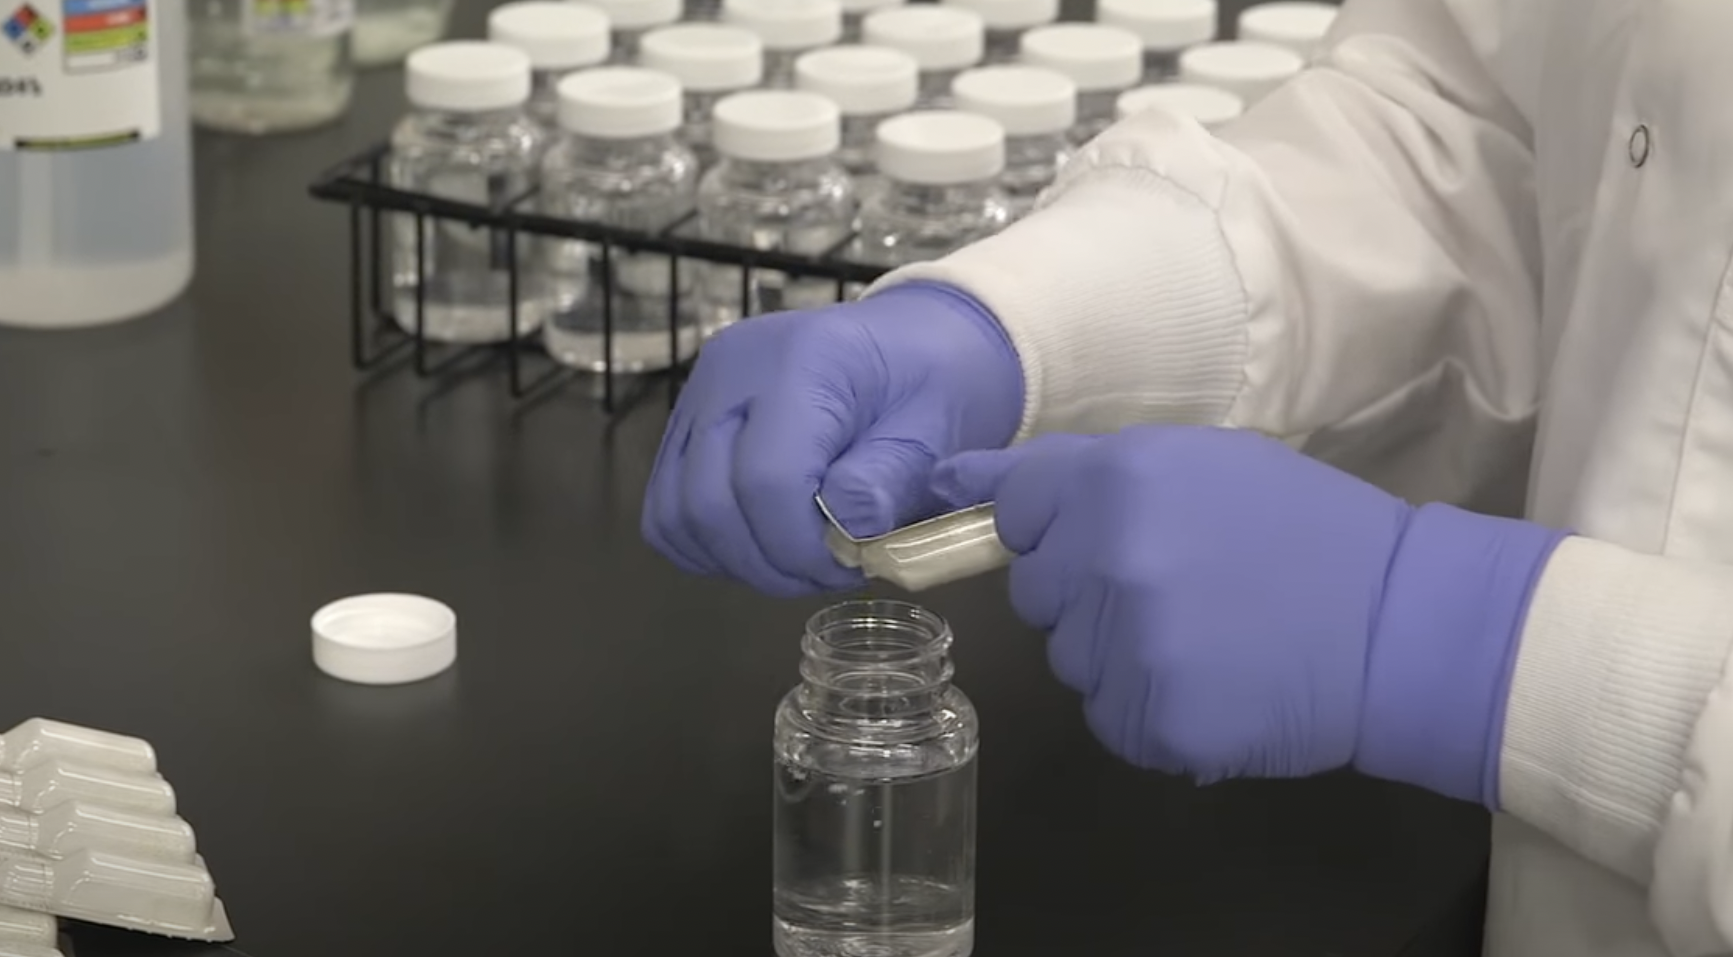
\includegraphics[width=1.0\textwidth]{figures/AddingReagent.png}
\caption{Adding Reagent}
\label{fig:Adding Reagent}
\end{figure}

\NP Place the lid back on the sample and shake well till the reagent has dissolved.

\NP Use a permanent felt tip marker to label your Quanti-tray with information identifying your sample. 

\NP Open the Quanti-tray by holding it at the top, with the well side facing your palm. Push the top edge of the Quanti-tray in with your free hand while squeezing the tray into a circle. Open the tray by gently pulling the foil tab away from the plastic side. Be careful not to tear the tab. Do not touch the inside of the tray. 

\begin{figure}
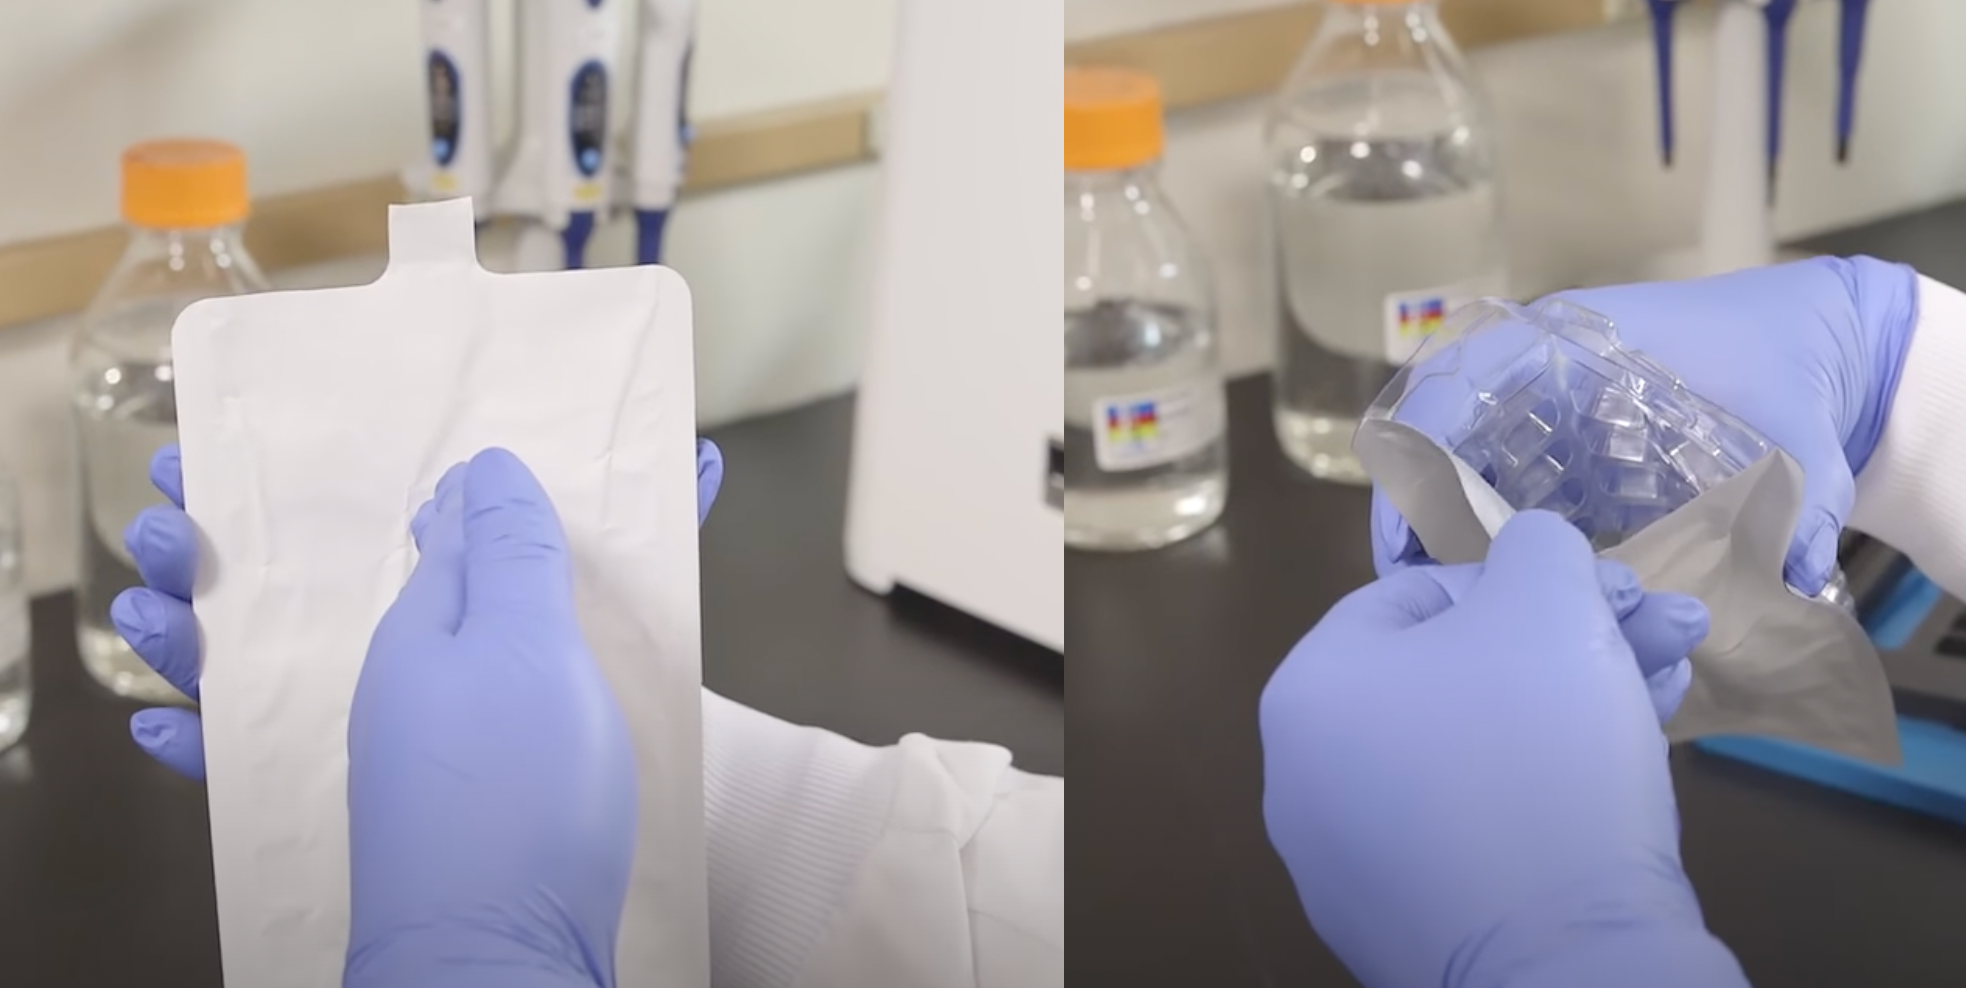
\includegraphics[width=1\textwidth]{figures/OpeningQuanti-Tray.png}
\caption{Opening and Pouring Sample into Quanti-Tray}
\label{fig:Adding Reagent}
\end{figure}

\clearpage

\NP Pour the sample mixture into the Quanti-tray, avoiding contact with the foil tab. Tap the small wells 2-3 times to release any air bubbles. Allow faom to settle.

\begin{figure}
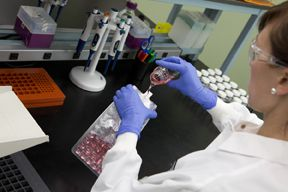
\includegraphics[width=0.7\textwidth]{figures/Step2.jpg}
\caption{Pouring Sampling into Quanti-Tray}
\end{figure}

\NP Place the filled Quanti-tray on the rubber insert, making sure each well fits its corresponding hole.

\NP Push the insert with the tray into the sealer, non foil tab end first, until the sealer grabs the tray and pulls it into the slot. If you need to reverse the motor, press and hold the reverse button. However, do not reverse the motor if the rubber insert is completely inside the sealer.
The sealer distributes the sample mixture into the Quanti-tray wells, seals the wells, and then partially ejects the sealed tray.

\begin{figure}[h]
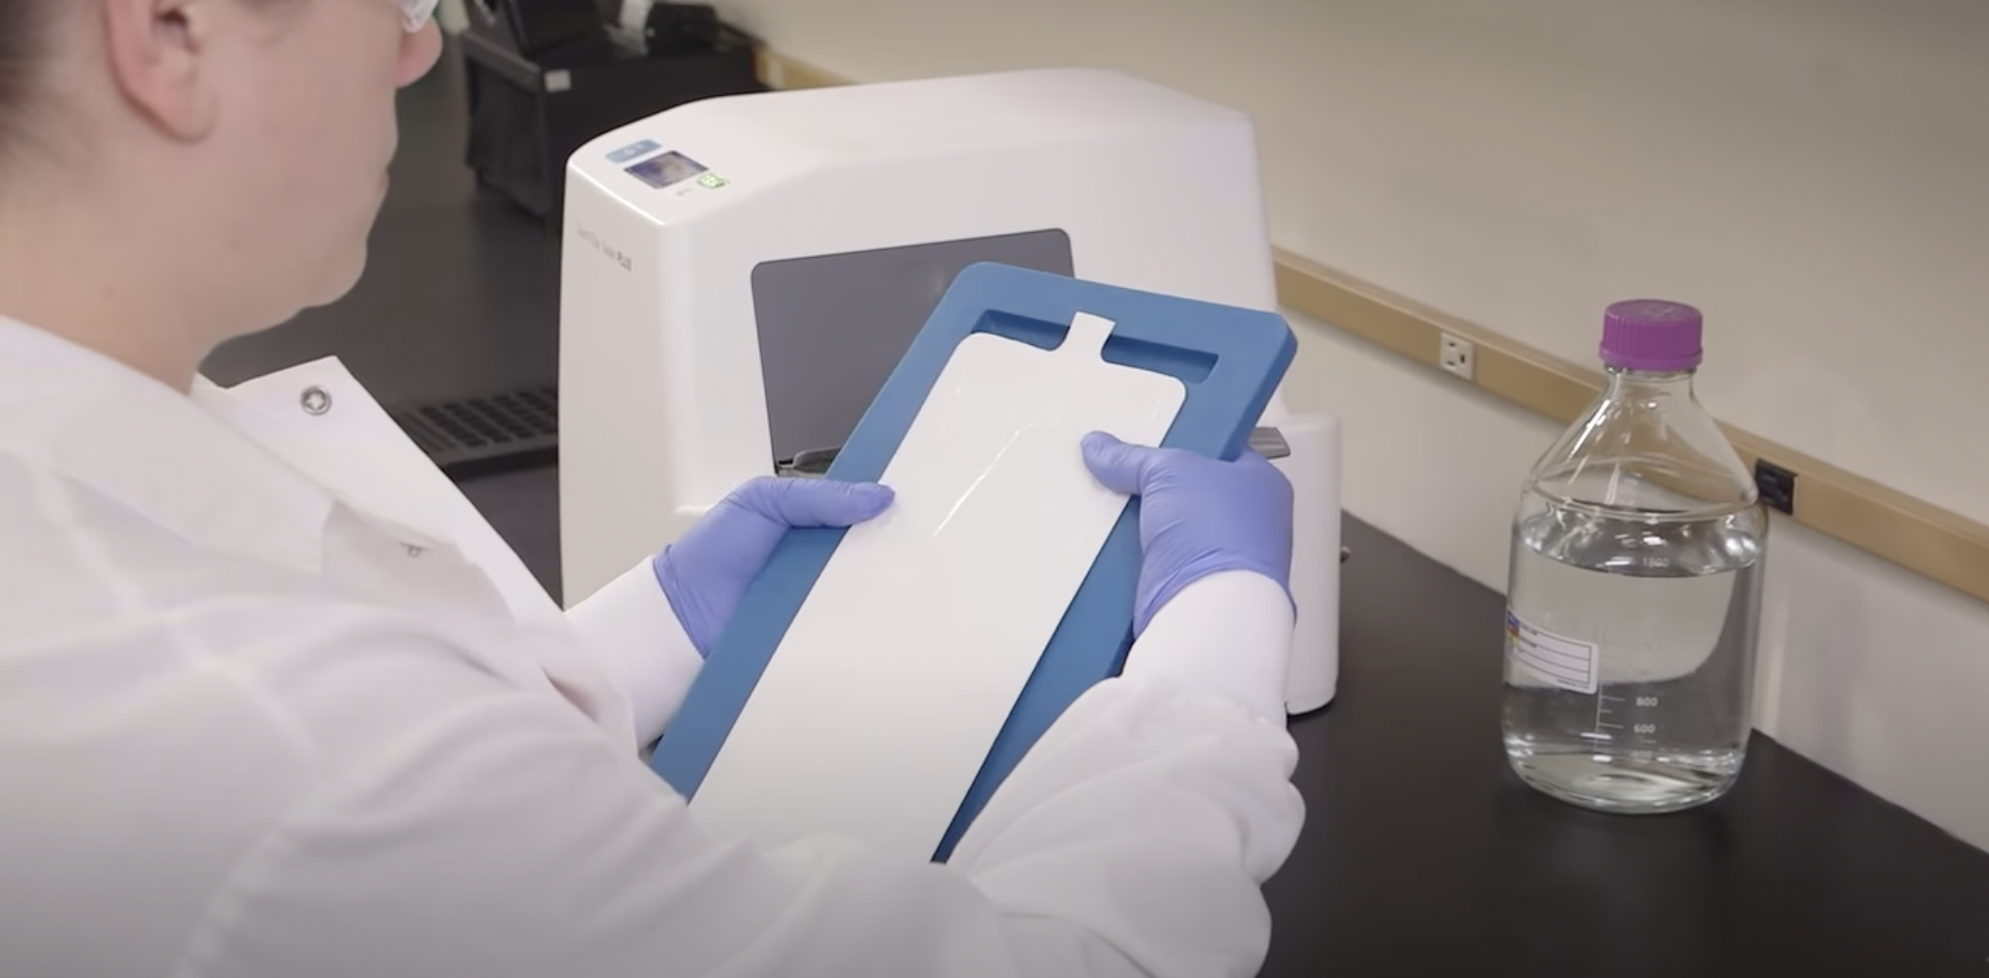
\includegraphics[width=0.7\textwidth]{figures/RubberInsert.png}
\caption{Pressing the Tray into the Rubber Insert}
\end{figure}

\NP Remove the rubber insert and tray from the sealer.

\NP Incubate the sealed tray for 24 hours at 35 \degree C $\pm$ 0.5 \degree C.
\NP After incubation, mark each yellow well with a permanent marker, including the large overflow well at the top. To determine the number of total coliforms, count the wells that are equal to or greater than the comparator, and then refer to the MPN.

\begin{figure}[h]
\centering
\includegraphics[width=0.6\textwidth]{figures/ColiformEcoliCount.png}
\caption{Counting Coliform and E Coli Wells (Be careful to avoid eye damage with  the use of the UV lamp.  )}
\end{figure}

\NP To determine the number of E Coli, view the Quanta-tray under a UV lamp. Count the fluorescent wells that are equal to, or greater than the comparator, and then refer to the MPN table.


\NP Use the Appendix Tables to calculate the MPN. 

\NP A count of 1–10 MPN/100 ml is regarded as low risk; 11–100 MPN/100 ml is medium risk. Finally, an E. coli count greater than 100 MPN/100 ml is judged high risk.


\NP Report results on the bench sheet.

\NP The completed bench sheet should be reviewed by the researcher, the
laboratory director and the QA manager. 

\subsection{Disposal}


\NP All materials must be autoclaved prior to disposal and workspaces
thoroughly disinfected.

\NP Dispose of media in accordance with Good Laboratory Practices.

%\clearpage
\section{Data Analysis and Calculations}

\NP For each sample analyzed, including quality control samples, record
the number of small and large positive wells and the MPN in the
appropriate places on the bench sheet (see below). Calculate
precision for duplicate analyses using equation 1.

\NP Equation 1. 

\begin{equation}
Precision (as RPD) = \frac{(A – B)*100}{(A + B)/2}
\end{equation}

Where: A = MPN from aliquot A and
 B = MPN from aliquot B 

\NP The following results should be observed:


\begin{table}
\caption{need to add caption}
		\begin{tabular}{ll}\hline

Organism                &  Result \\ \hline \hline
Escherichia coli        & Yellow wells, fluorescence \\
Klebsiella pneumoniae   & Yellow wells, no fluorescence \\
Pseudomonas aeruginosa  & Clear wells, no fluorescence \\
Method Blank            & Clear wells, no fluorescence \\ \hline
  \end{tabular}
\end{table}


\section{QC/QA Criteria}

\subsection{Using Standards}

\NP TBD

\subsection{Data assessment and acceptable criteria}

\NP The analyst should review all data for correctness (e.g., use of MPN table).

%\NP Precision values are calculated for pairs of duplicate analyses.

\NP Record the precision values as RPD on the bench sheet.

\NP The desired precision is ± 20% (RPD).

\NP The desired detection limit is 1 MPN/100mL

\NP The completed bench sheet is reviewed by the analyst's supervisor or the
QVIR Lab Director 


\subsection{Corrective actions for out-of-control or unacceptable data}

\NP The results for precision and blank data are compared to the
acceptable values for this analysis; ± 20\% and 1 MPN/100mL,
respectively.

\NP If a precision value exceeds 20\% then the analyst should write in the
comments section of the bench sheet: “These data are associated
with an out-of-control duplicate analysis. The UCL = 20\%.” Note:
“UCL” is the Upper Control Limit (i.e., 20%).

\NP If a blank value exceeds 1 MPN/100mL then the analyst should write
in the comments section of the bench sheet: “These data are
associated with a blank value that exceeds the detection limit of 1
MPN/100mL.”

\NP The samples cannot be reanalyzed because the sample volume will be
depleted after the initial analysis.

\NP  If data are unacceptable for any reason, the analyst should review
their analytical technique prior to conducting this analysis again. 

\subsection{Disposal}


\NP All materials must be autoclaved prior to disposal and workspaces
thoroughly disinfected.

\NP Dispose of media in accordance with Good Laboratory Practices.

\section{Trouble Shooting}

TBD!!! 


\section{References}

\NP APHA, AWWA. WEF. (2012) Standard Methods for examination of water and wastewater. 22nd American Public Health Association (Eds.). Washington. 1360 pp. (2014).

\appendix

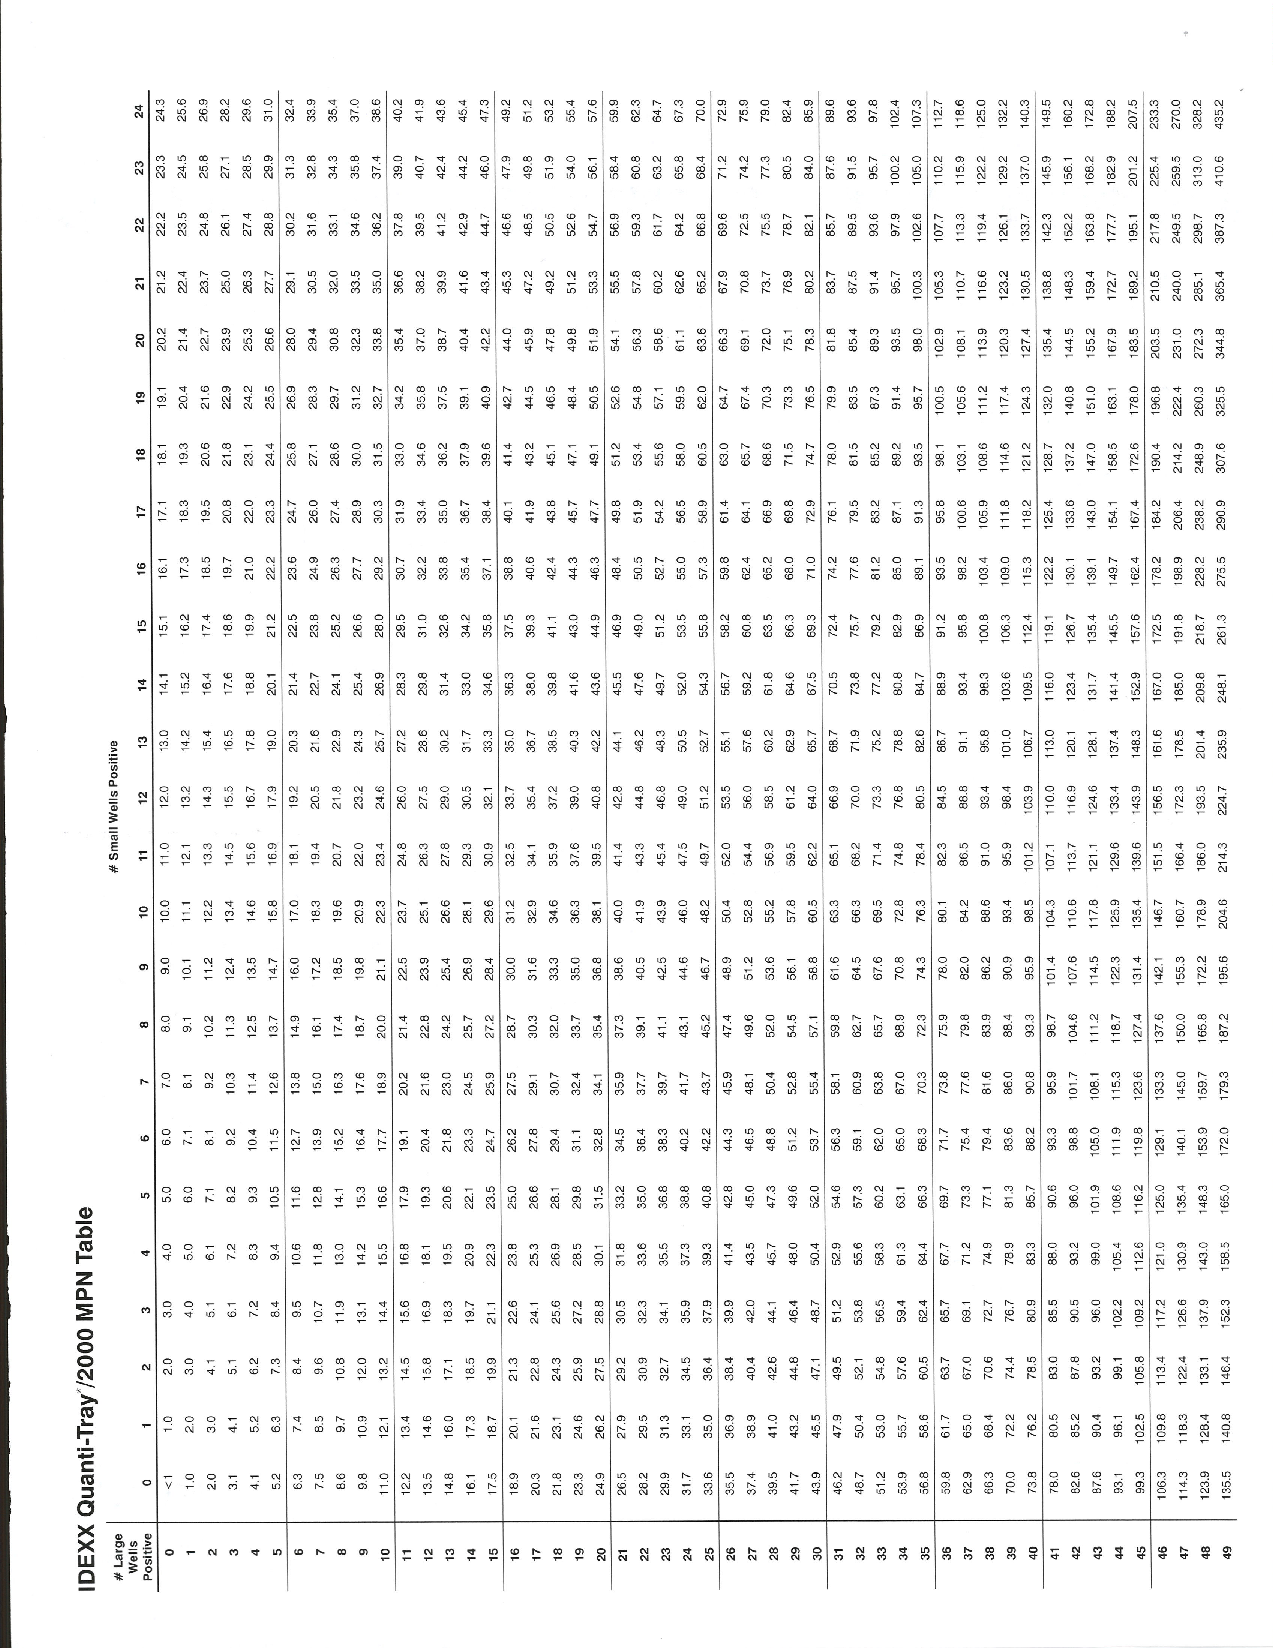
\includepdf{0312_002}
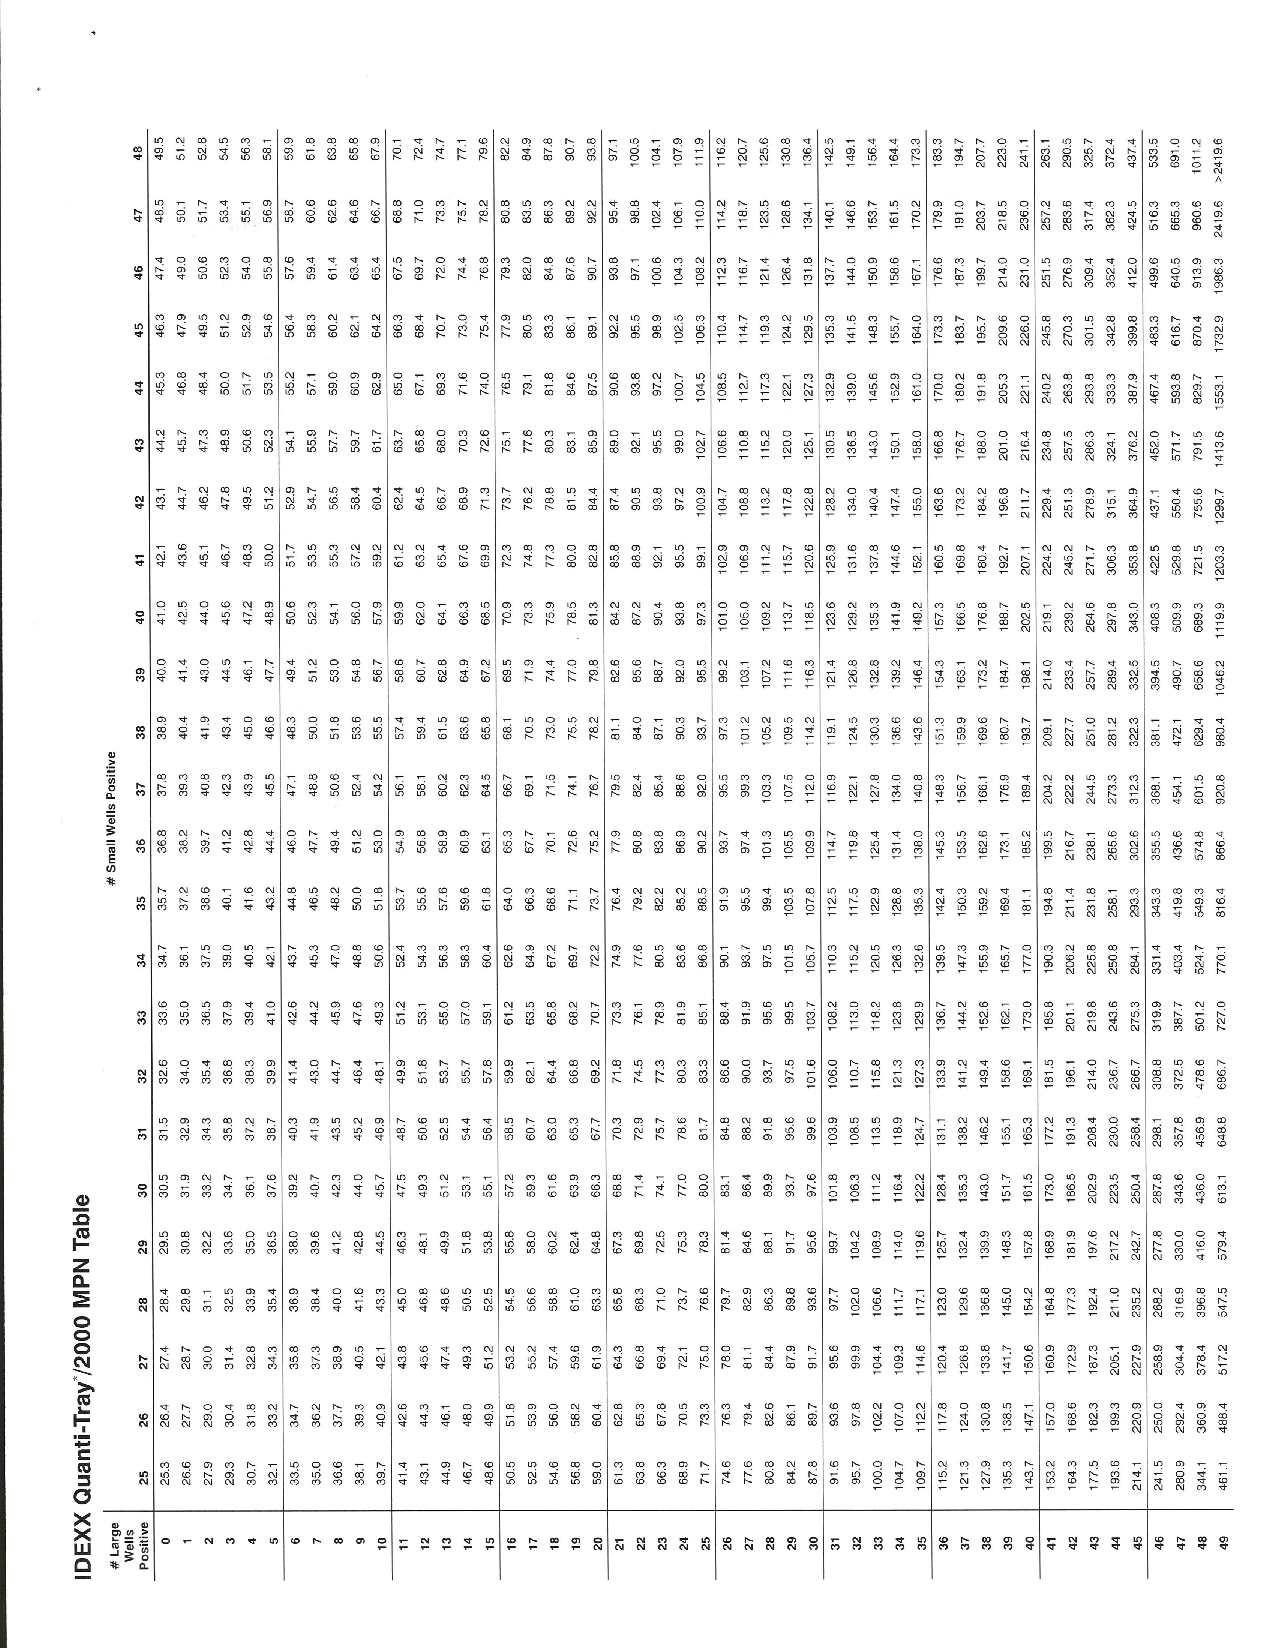
\includepdf{0312_001}


\end{document}
